\documentclass[11pt]{article}
\usepackage[cm]{fullpage}
\usepackage{mathtools} %includes amsmath
\usepackage{amssymb}
\usepackage{simplewick}
\usepackage{soul}
\usepackage{bm}
\usepackage{amsthm}
\usepackage{amsfonts}
\usepackage{hyperref}
%greek letters
\newcommand{\f}{\ensuremath{\phi}}
\newcommand{\F}{\ensuremath{\Phi}}
\newcommand{\w}{\ensuremath{\omega}}
\newcommand{\W}{\ensuremath{\Omega}}
\renewcommand{\th}{\ensuremath{\theta}}
\newcommand{\Th}{\ensuremath{\Theta}}
\newcommand{\y}{\ensuremath{\psi}}
\newcommand{\Y}{\ensuremath{\Psi}}
\newcommand{\eps}{\ensuremath{\bm\epsilon}}
\newcommand{\E}{\ensuremath{\mathcal{E}}}
\newcommand{\e}{\ensuremath{\bm{\varepsilon}}}
\newcommand{\g}{\ensuremath{\gamma}}
\newcommand{\G}{\ensuremath{\Gamma}}
\newcommand{\la}{\ensuremath{\lambda}}
\newcommand{\La}{\ensuremath{\Lambda}}
\newcommand{\si}{\ensuremath{\sigma}}
\newcommand{\Si}{\ensuremath{\Sigma}}
\renewcommand{\d}{\ensuremath{\delta}}
\newcommand{\D}{\ensuremath{\Delta}}
\newcommand{\A}{\ensuremath{\alpha}}
\newcommand{\B}{\ensuremath{\beta}}
\newcommand{\K}{\ensuremath{\kappa}}
\newcommand{\rh}{\ensuremath{\rho}}
\newcommand{\x}{\ensuremath{\chi}}
\newcommand{\ta}{\ensuremath{\tau}}
\newcommand{\z}{\ensuremath{\zeta}}
%ornaments
\renewcommand{\eth}{\ensuremath{^\text{th}}}
\newcommand{\rst}{\ensuremath{^\text{st}}}
\newcommand{\ond}{\ensuremath{^\text{nd}}}
\newcommand{\ord}[1]{\ensuremath{^{(#1)}}}
\newcommand{\dg}{\ensuremath{^\dagger}}
\newcommand{\bigo}{\ensuremath{\mathcal{O}}}
\newcommand{\tl}{\ensuremath{\tilde}}
\newcommand{\ol}[1]{\ensuremath{\overline{#1}}}
\newcommand{\op}[1]{\ensuremath{ \hat{#1} } }
%text
\newcommand{\occ}{\ensuremath{\mrm{occ}}}
\newcommand{\vir}{\ensuremath{\mrm{vir}}}
\newcommand{\spn}{\ensuremath{\mrm{span}}}
\renewcommand{\ker}{\ensuremath{\mrm{ker}}}
\newcommand{\vac}{\ensuremath{\kt{\mrm{vac}}}}
\newcommand{\sgn}{\ensuremath{\mrm{sgn}}}
\newcommand{\jsq}{\ensuremath{\op{\bo{J}}^2}}
\newcommand{\jbo}{\ensuremath{\op{\bo{J}}}}
\newcommand{\jup}{\ensuremath{\op{J}_+}}
\newcommand{\jdn}{\ensuremath{\op{J}_-}}
\newcommand{\jz}{\ensuremath{\op{J}_z}}
\newcommand{\lsq}{\ensuremath{\op{\bo{L}}^2}}
\newcommand{\lbo}{\ensuremath{\op{\bo{L}}}}
\newcommand{\lup}{\ensuremath{\op{L}_+}}
\newcommand{\ldn}{\ensuremath{\op{L}_-}}
\newcommand{\lz}{\ensuremath{\op{L}_z}}
\newcommand{\Ssq}{\ensuremath{\op{\bo{S}}^2}}
\newcommand{\Sbo}{\ensuremath{\op{\bo{S}}}}
\newcommand{\Sup}{\ensuremath{\op{S}_+}}
\newcommand{\Sdn}{\ensuremath{\op{S}_-}}
\newcommand{\Sz}{\ensuremath{\op{S}_z}}
\newcommand{\Nu}{\ensuremath{\mathrm{Nu}}}
%dots
\newcommand{\ld}{\ensuremath{\ldots}}
\newcommand{\cd}{\ensuremath{\cdots}}
\newcommand{\vd}{\ensuremath{\vdots}}
\newcommand{\dd}{\ensuremath{\ddots}}
\renewcommand{\sp}{\ensuremath{\ \ \ \ \ \ }}
%fonts
\newcommand{\mc}[1]{\ensuremath{\mathcal{#1}}}
\newcommand{\bo}[1]{\ensuremath{\mathbf{#1}}}
\newcommand{\mrm}[1]{\ensuremath{\mathrm{#1}}}
%fractions, derivatives, parentheses, brackets, etc.
\newcommand{\pr}[2]{\ensuremath{\left( #2 \right)^{#1}}}
\newcommand{\fr}[2]{\ensuremath{ \dfrac{#1}{#2} }}
\newcommand{\tr}[1]{\ensuremath{\text{tr}[#1]}}
\newcommand{\pd}[2]{\ensuremath{\dfrac{\partial#1}{\partial #2}}}
\newcommand{\pt}{\ensuremath{\partial}}
\newcommand{\br}[1]{\ensuremath{ \langle #1 |}}
\newcommand{\kt}[1]{\ensuremath{ | #1 \rangle}}
\newcommand{\ip}[1]{\ensuremath{\langle #1\rangle}}
\newcommand{\NO}[1]{\ensuremath{{\bm{:}}#1{}{\bm{:}}}}
\newcommand{\cmtr}[2]{\ensuremath{[\cdot,#2]^{#1}}}
\newcommand{\cmtl}[2]{\ensuremath{[#2,\cdot]^{#1}}}
%structures
\newcommand{\bne}{\begin{equation}}
\newcommand{\ene}{\end{equation} }
\newcommand{\eqn}[1]{(\ref{#1})}
\newcommand{\ma}[1]{\ensuremath{\left(\begin{matrix} #1 \end{matrix}\right)}}
\newcommand{\ar}[1]{\ensuremath{\begin{matrix} #1 \end{matrix}}}
\newcommand{\miniar}[1]{\ensuremath{\begin{smallmatrix}#1\end{smallmatrix}}}
%contractions
\newcommand{\C}[6]{\ensuremath{\contraction[#1ex]{#2}{#3}{#4}{#5}#2#3#4#5#6}}
\newcommand{\CT}[5]{\ensuremath{\contraction[#1ex]{#2}{#3}{#4}{#5}}}
\newcommand{\Cttt}[4]{\ensuremath{\contraction[2.5ex]{#1}{#2}{#3}{#4}}}
\newcommand{\Ctt}[4]{\ensuremath{\contraction[2.0ex]{#1}{#2}{#3}{#4}}}
\newcommand{\Ct}[4]{\ensuremath{\contraction[1.5ex]{#1}{#2}{#3}{#4}}}
\newcommand{\Cb}[5]{\ensuremath{\contraction[1ex]{#1}{#2}{#3}{#4}#1#2#3#4#5}}
\newcommand{\cT}[5]{\ensuremath{\bcontraction[#1ex]{#2}{#3}{#4}{#5}}}
\newcommand{\cttt}[4]{\ensuremath{\bcontraction[2.5ex]{#1}{#2}{#3}{#4}}}
\newcommand{\ctt}[4]{\ensuremath{\bcontraction[2.0ex]{#1}{#2}{#3}{#4}}}
\newcommand{\ct}[4]{\ensuremath{\bcontraction[1.5ex]{#1}{#2}{#3}{#4}}}
\newcommand{\cb}[5]{\ensuremath{\bcontraction[1ex]{#1}{#2}{#3}{#4}#1#2#3#4#5}}
%math sections
\makeatletter
\newtheoremstyle{indented}{3pt}{3pt}{\small \setlength{\leftskip}{3em}\addtolength{\@totalleftmargin}{2.5em}\setlength{\rightskip}{3em}}{}{\bfseries}{:}{.5em}{\large \it \thmname{#1}\thmnumber{ #2} \rm}
\makeatother
\theoremstyle{indented}
\newtheorem{dfn}{Definition}[section]
\newtheorem{prf}{Proof}[section]
\newtheorem{rmk}{Remark}[section]



\title{Programming Project 3 Theory (Part 1)\\
\textit{Hartree-Fock theory}}
\date{}
\author{}

\begin{document}
\maketitle
\vspace{-1cm}

\noindent
The goal of electronic structure theory is to solve the ``clamped-nuclei'' Schr\"odinger equation
\begin{align}
\label{se}
	\op{H}_e\Y_K
=&\
	E_K\Y_K
\\
	\op{H}_e
=&\
\sum_{A<B}
	\fr{Z_AZ_B}{|\bo{R}_A-\bo{R}_B|}
-\fr{1}{2}\sum_i
	\nabla_i^2
-\sum_A\sum_i
	\fr{Z_A}{|\bo{R}_A-\bo{r}_i|}
+\sum_{i<j}
	\fr{1}{|\bo{r}_i-\bo{r}_j|}
\end{align}
with an optimal balance of accuracy and efficiency for the problem of interest.
The most accurate solution possible for a given basis set (cc-pVXZ, DZP, ANO1, etc.) results from expanding the wavefunction
\begin{align}
\label{n-e-expansion}
	\Y_K
=&\
	\sum_P
	\F_P c_{PK}
\end{align}
in terms of all possible Slater determinants (the $n$-electron basis functions $\{\F_P\}$) that can be formed from an orthonormal one-electron basis (spin-orbitals $\{\y_p\}$), and solving for the coefficients as eigenvectors of a matrix representation of $\op{H}_e$ in the $n$-electron basis, $(\bo{H})_{PQ}=\ip{\F_P|\op{H}_e|\F_Q}$.
This is called the {\it full configuration-interaction} (FCI) solution.

Any one-electron basis spans the same ``function space'' as the AO basis set itself, and the full $n$-electron basis $\{\F_P\}$ spans the same space of $n$-electron functions regardless of how one forms spin orbitals from the AO basis set.
As a result, one obtains the same FCI solution for any choice of spin-orbitals.
In general, however, FCI solutions are completely unfeasible for basis sets of sufficient size to approach the complete basis set limit.
One can think of this as a simple counting problem: if there are $m$ functions in the AO basis, then there are $2m$ spin MOs in the one-electron basis \footnote{$m$ $\A$-orbitals and $m$ $\B$-orbitals.}, and there are ``$2m$ choose $n$'' \footnote{The number of unique sets of $n$ marbles that can be drawn from a bag of $2m$ marbles.  See \url{http://en.wikipedia.org/wiki/Combination}}
\begin{align*}
\ma{2m\\n}\equiv\fr{(2m)!}{n!(2m-n)!}
\end{align*}
unique Slater determinants in the $n$-electron basis that can be formed from the spin MOs.
The upshot is that we typically have to omit some of the Slater determinants in our $n$-electron basis in order to make progress toward obtaining a solution in a reasonable amount of time.

As soon as we truncate our Slater determinant expansion (\ref{n-e-expansion}), our choice of spin MOs makes a significant difference in the quality of our results.
In particular, we need to choose our set of one-electron functions to minimize the number of Slater determinants it takes to ``get close to'' the exact wavefunction.


\section*{Defining the problem}
It can be shown that the exact ground- and excited-state wavefunctions of a system are stationary points of the Hamiltonian expectation value $\ip{\op{H}_e}=\ip{\Y|\op{H}_e|\Y}$ with $\Y$ constrained to be normalized.
That is, optimizing $\ip{\Y|\op{H}_e|\Y}$ by varying $\Y(1,\ld,n)$ subject only to the constraint $\ip{\Y|\Y}=1$ is equivalent to solving the Schr\"odinger equation.
When we further constrain the form of $\Y$, this is no longer true (i.e.\ we will generally {\it not} get an exact eigenfunction of $\op{H}_e$).
However, this {\it does} generally allow us to get the best approximation to $\Y$ subject to the additional constraints.

In order to make the Slater determinant expansion (\ref{n-e-expansion}) converge with a relatively small number of $\F_P$'s, we wish to find the \ul{best single-determinant approximation to $\Y$}.
That is, we wish to optimize
\begin{align}
	\ip{\F|\op{H}_e|\F}
\sp\sp
	\F(1,\ld,n)
=
\fr{1}{\sqrt{n!}}
\left|\ar{
	\y_1(1)&\y_2(1)&\cd&\y_n(1)\\
	\y_1(2)&\y_2(2)&\cd&\y_n(2)\\
	\vd    &\vd    &\dd&\vd    \\
	\y_1(n)&\y_2(n)&\cd&\y_n(n)}\right|
\end{align}
with respect to variation of the orbitals $\{\y_p\}$, enforcing the normalization constraint by keeping the spin orbitals orthonormal.
This orbital optimization procedure is called the {\it Hartree-Fock method}.

Once we have solved this optimization problem, the expectation value $\ip{\F|\op{H}_e|\F}$ is itself a good first approximation to the electronic energy.
Indeed, the Hartree-Fock method usually recovers the bulk of the electronic energy.\footnote{Although the importance of the remaining ``correlation energy'' cannot possibly be underestimated!}
More importantly, however, when we use this new set of Hartree-Fock MOs, $\{\y_p\}$, the FCI expansion tends to converge much more quickly to the true wavefunction.
Specifically, when we rewrite the determinant expansion (\ref{n-e-expansion}) in terms of single $\{\F_i^a\}$, double $\{\F_{ij}^{ab}\}$, triple $\{\F_{ijk}^{abc}\}$, etc.\ replacements \footnote{It is typical to use dummy indices $i,j,k,l$ to count over the orbitals in the reference determinant $\F$ -- the ``occupied orbitals'' -- and to use $a,b,c,d,$ to count over the orbitals not contained in $\F$ -- the ``unoccupied'' or ``virtual orbitals.''  Dummy indices $p,q,r,s$ are generally used to count over the full set of spin MOs, whether occupied or not.} of the orbitals in the Hartree-Fock determinant $\F$ with the remaining orbitals in the basis
\begin{align}
	\Y
=
	\F
+
	\sum_{\miniar{a\\i}}
	\F_i^ac_i^a
+
	\sum_{\miniar{a<b\\i<j}}
	\F_{ij}^{ab}c_{ij}^{ab}
+
	\sum_{\miniar{a<b<c\\i<j<k}}
	\F_{ijk}^{abc}c_{ijk}^{abc}
+\ld
\end{align}
the coefficients tend to be very small, and are often virtually negligible for higher than quadruple replacements.

\section*{Derivation}
What follows is a derivation of the canonical Hartree-Fock equations, which define the Slater determinant $\F$ that is a stationary point of the Hamiltonian expectation value $\ip{\F|\op{H}_e|\F}$.
A discussion of some of the background needed to understand why this derivation works is given in a series of appendices at the end.

\subsection*{Components of $\op{H}_e$}
The electronic Hamiltonian $\op{H}_e$ contains zero-, one-, and two-electron operators
\begin{align}
	\op{H}_e
=&\
	V_\Nu
+
	\sum_i
	\op{h}(i)
+
	\sum_{i<j}
	\op{g}(i,j)
\\
	V_\Nu
\equiv&\
	\sum_{A<B}\fr{Z_AZ_B}{|\bo{R}_A-\bo{R}_B|}
\\
	\op{h}(i)
\equiv&\
-\fr{1}{2}
	\nabla_i^2
+\sum_A
	\fr{Z_A}{|\bo{r}_i-\bo{R}_A|}
\\
	\op{g}(i,j)
\equiv&\
	\fr{1}{|\bo{r}_i-\bo{r}_j|}
\end{align}
which can be identified by the number of electron coordinates upon which they act.

\subsection*{Single-determinant expectation value of $\op{H}_e$}
The single-determinant expectation value of the electronic Hamiltonian is given by the first Slater rule
\begin{align}
	\ip{\F|\op{H}_e|\F}
=
\sum_{i}^n
	\ip{\y_i|\op{h}|\y_i}
+\fr{1}{2}\sum_{ij}^n
	\ip{\y_i\y_j||\y_i\y_j}
\end{align}
where the one- and two-electron integrals ($\ip{\y_p|\op{h}|\y_q}$ and $\ip{\y_p\y_q||\y_r\y_s}$, respectively) are defined as follows.
\begin{align}
\label{oei}
	\ip{\y_p|\op{h}|\y_q}
\equiv&\
\int d(1)
	\y_p^*(1)
	\op{h}(1)
	\y_q(1)
\\
\label{tei}
	\ip{\y_p\y_q|\y_r\y_s}
\equiv&\
\int d(1,2)
	\y_p^*(1)\y_q^*(2)
	\op{g}(1,2)
	\y_r(1)\y_s(2)
\sp\sp
	\ip{\y_p\y_q||\y_r\y_s}
\equiv
	\ip{\y_p\y_q|\y_r\y_s}
-
	\ip{\y_p\y_q|\y_s\y_r}
\end{align}




\subsection*{The Hartree-Fock Lagrangian}
We wish to optimize the single-determinant expectation value of $\op{H}_e$
\begin{align}
	\ip{\F|\op{H}_e|\F}
=
\sum_{i=1}^n
	\ip{\y_i|\op{h}|\y_i}
+\fr{1}{2}\sum_{i,j=1}^n
	\ip{\y_i\y_j||\y_i\y_j}
\end{align}
with respect to variation in of the orbitals $\{\y_i\}$, subject to the constraint that the orbitals remain orthonormal.
\begin{align}
	\ip{\y_i|\y_j}=\d_{ij}
\end{align}
This means that our Lagrangian functional \footnote{A functional is just a function of a function -- i.e.\ some rule $F$ that maps a function $f$ to a number $F[f]$.  Definite integrals are probably the most common example.} takes the form
\begin{align}
\label{lagrangian}
	\mc{L}[\{\y_i\},\{\eps_{ij}\}]
=
\sum_{i=1}^n
	\ip{\y_i|\op{h}|\y_i}
+\fr{1}{2}\sum_{i,j=1}^n
	\ip{\y_i\y_j||\y_i\y_j}
-\sum_{i,j=1}^n
	\eps_{ij}(\ip{\y_i|\y_j}-\d_{ij})
\end{align}
where $\{\eps_{ij}\}$ are our Lagrangian multipliers for the orthonormality constraint (see appendix \ref{constrained-optimization} for a brief explanation the Lagrangian approach to constrained optimization).


\subsection*{Hartree-Fock Equations}
In order to determine the stationarity condition for the spin MOs, we require that (see \ref{optimizing-functionals})
\begin{align}
\left.
	\fr{d\mc{L}[\y_k+\e \eta]}{d\e}
\right|_{\e=0}
\overset{!}=
	0
\end{align}
holds for every orbital $\y_k$.
That is, we require that for all of the orbitals $\y_1,\ld,\y_n$ in the Slater determinant $\F$, adding a little bit of some arbitrary function $\eta=\eta(\bo{r},m_s)$ doesn't change the Lagrangian.

Separating the terms in (\ref{lagrangian}) involving one of the orbitals $\y_k$ from the remaining terms, we can write
\begin{align*}
	\mc{L}
=&\
	\ip{\y_k|\op{h}|\y_k}
+\sum_i
	\ip{\y_k\y_i||\y_k\y_i}
-\sum_i
	\eps_{ki}(\ip{\y_k|\y_i}-\d_{ki})
-\sum_i
	\eps_{ik}(\ip{\y_i|\y_k}-\d_{ik})
\\&\
+\sum_{i\neq k}
	\ip{\y_i|\op{h}|\y_i}
+\fr{1}{2}\sum_{i\neq k,j\neq k}
	\ip{\y_i\y_j||\y_i\y_j}
-\sum_{i\neq k,j\neq k}
	\eps_{ij}(\ip{\y_i|\y_j}-\d_{ij})
\end{align*}
using the fact that $\ip{\y_k\y_i||\y_k\y_i}=\ip{\y_i\y_k||\y_i\y_k}$, which can be seen by exchanging dummy variables of integration in the integral (\ref{tei}).
The functional derivative for varying $\y_k$ is then
\begin{align*}
&\left.
	\fr{d\mc{L}[\y_k+\e \eta]}{d\e}
\right|_{\e=0}
= \\
&
\left.
\fr{d}{d\e}\pr{}{
	\ip{\y_k+\e\eta|\op{h}|\y_k+\e\eta}
+\sum_i
	\ip{(\y_k+\e\eta)\y_i||(\y_k+\e\eta)\y_i}
-\sum_i
	\eps_{ki}\ip{\y_k+\e\eta|\y_i}
-\sum_i
	\eps_{ik}\ip{\y_i|\y_k+\e\eta}	   }
\right|_{\e=0}
\end{align*}
where we have dropped all terms not involving $\e$ (including the $\d_{ik}$s), since their derivatives vanish.
Evaluating the derivative and plugging in $\e=0$, we get
\begin{align*}
\left.
	\fr{d\mc{L}[\y_k+\e \eta]}{d\e}
\right|_{\e=0}
=&\
	\ip{\eta|\op{h}|\y_k}
+\sum_i
	\ip{\eta\y_i||\y_k\y_i}
-\sum_i
	\eps_{ki}
	\ip{\eta|\y_i}
+
	\ip{\y_k|\op{h}|\eta}
+\sum_i
	\ip{\y_k\y_i||\eta\y_i}
-\sum_i
	\eps_{ik}
	\ip{\y_i|\eta}
\end{align*}
The first two terms can be rewritten as \footnote{Defining $\ip{\y_p(2)|\op{g}(1,2)|\y_q(2)}\equiv\int d(2) \y_p^*(2)\op{g}(1,2)\y_q(2)$}
\begin{align*}
	\ip{\eta|\op{h}|\y_k}
+\sum_i
	\ip{\eta\y_i||\y_k\y_i}
=
\int d(1)
	\eta^*(1)
	\pr{}{
		\op{h}(1)
	+\sum_i
		\ip{\y_i(2)|\op{g}(1,2)(1-\op{P}(1,2))|\y_i(2)}  }
	\y_k(1)
\end{align*}
where $\op{P}(1,2)$ is an ``operator'' that swaps the coordinates of the two one-electron functions on its right (prior to integration).
\footnote{This really just a notational trick to allow us to use the short-hand $\y_i(1)\y_j(2)-\y_j(1)\y_i(2)\equiv(1-\op{P}(1,2))\y_i(1)\y_j(2)$ which could just as easily be done by instead defining an ``index-permuter'' $\op{P}_{ij}$ to swap the orbital indices.}
The term in parenetheses is called the {\it Fock operator}
\footnote{You have probably seen this written as
$\op{f}(1)=\op{h}(1)+\sum_i(\op{J}_i(1)-\op{K}_i(1))$
where $\op{J}_i(1)\equiv\ip{\y_i(2)|\op{g}(1,2)|\y_i(2)}$ and $\op{K}_i\equiv\ip{\y_i(2)|\op{g}(1,2)\op{P}(1,2)|\y_i(2)}$ are called the Coloumb and exchange operators.}
\begin{align}
\label{fock}
	\op{f}(1)
\equiv
	\op{h}(1)
+\sum_i
	\ip{\y_i(2)|\op{g}(1,2)(1-\op{P}(1,2))|\y_i(2)}
\end{align}
which, note, is really an operator functional of the orbitals $\op{f}=\op{f}[\y_1,\ld,\y_n]$.

With this new operator, our stationarity condition takes the form
\begin{align*}
\int d(1)\eta^*(1)\pr{}{
	\op{f}(1)\y_k(1)
-\sum_i
	\eps_{ki}
	\y_i(1)  }
+\int d(1)\pr{}{
	\y_k^*(1)\op{f}(1)
-\sum_i
	\y_i^*(1)
	\eps_{ik}  }
	\eta(1)
\overset{!}=0
\end{align*}
where we see that the second term is the complex conjugate of the first.
By the Fundamental Lemma of Calculus of Variations (see appendix \ref{flcv}), this condition is equivalent to requiring
\begin{align}
\label{cond1}
	\op{f}(1)\y_k(1)-\sum_i \eps_{ki}\y_i(1) \overset{!}=&\ 0
\\
\label{cond2}
	\op{f}(1)\y_k^*(1)-\sum_i \eps_{ik}\y_i^*(1) \overset{!}=&\ 0
\end{align}
where we have used the fact that the Fock operator is Hermitian, so that $\ip{\y_k|\op{f}\eta}=\ip{\op{f}\dg\y_k|\eta}=\ip{\op{f}\y_k|\eta}$.
Subtracting the complex conjugate of equation (\ref{cond2}) from equation (\ref{cond1}) gives
\begin{align*}
\sum_i
	(\eps_{ki}-\eps_{ik}^*)\y_i(1)
\overset{!}=
	0
\end{align*}
and, since the orbitals $\{\y_i\}$ are linearly independent, \footnote{\url{http://en.wikipedia.org/wiki/Linear_independence\#Definition}}
this tells us that
\begin{align*}
	\eps_{k1}-\eps_{1k}^*=\cd=\eps_{kn}-\eps_{nk}^*=0
\end{align*}
i.e.\ the matrix of Lagrange multipliers $\{\eps_{ij}\}$ must be Hermitian.

This gives us a new set of conditions for stationarity of $\ip{\F|\op{H}_e|\F}$ subject to the constraint $\ip{\y_i|\y_j}=\d_{ij}$
\begin{align}
\label{hf-noncanonical}
	\op{f}\y_i
\overset{!}=&\
	\sum_j \eps_{ij}\y_j
\sp
	\eps_{ij}\overset{!}=\eps_{ji}^*
\end{align}
which is one form of the {\it Hartree-Fock equations}.
We can show that this set of equations can be partially decoupled \footnote{We can never fully decouple them, because the Fock operator depends on all of the orbitals.}
by diagonalizing the multiplier matrix to give a series of eigenvalue equations $\op{f}\y_i=\eps_i\y_i$, known as the {\it canonical Hartree-Fock equations}.

\subsection*{Canonical Hartree-Fock Equations}
Equation (\ref{hf-noncanonical}) can be written in matrix form as
\begin{align}
\label{hf-noncanonical-matrix}
	\op{f}\bm\y
\overset{!}=
	\eps\bm\y
\sp
	\eps=\eps\dg
\end{align}
where we have defined a matrix of Lagrange multipliers and a vector of orbitals.
\begin{align}
	\eps
=
	\ma{\eps_{11}&\cd&\eps_{1n}\\
		\vd&\dd&\vd\\
		\eps_{n1}&\cd&\eps_{nn}}
\sp
	\bm\y
=
	\ma{\y_1\\\vd\\\y_n}
\end{align}
Since $\eps$ is a Hermitian matrix, it can be diagonalized by a unitary \footnote{\url{http://en.wikipedia.org/wiki/Unitary_matrix}} transformation $\bo{U}$.
\begin{align}
	\eps
=
	\bo{U}\tl\eps\bo{U}\dg
\end{align}
Inserting this decomposition into equation (\ref{hf-noncanonical-matrix}) and multiplying both sides from the left by $\bo{U}\dg$, we get
\begin{align*}
	\op{f}(\bo{U}\dg\bm\y)
=
	\tl\eps(\bo{U}\dg\bm\y)
\end{align*}
which shows that the problem can be put into canonical form by using a new set of orbitals $\tl{\bm\y}=\bo{U}\dg\bm\y$ formed from $\y_1,\ld,\y_n$ as 
\begin{align}
	\tl\y_i
=
	\sum_{j=1}^n U_{ji}^*\y_j
\end{align}
We can show that this ``re-mixing'' of the orbitals in $\F$ leaves the Fock operator $\op{f}$ and the expectation value $\ip{\F|\op{H}_e|\F}$ unchanged, while also preserving orbital orthonormality (see \ref{hf-invariance}).

Dropping the tildes, the {\it canonical Hartree-Fock equations} can be written as
\begin{align*}
	\op{f}\y_i
=
	\eps_i\y_i
\sp
	i=1,\ld,n
\end{align*}
where $\eps_i$ is an element of the diagonal multiplier matrix and the requirement that $\eps=\eps\dg$ now simply means that each $\eps_i$ is real, $\eps_i=\eps_i^*$.
Note that these equations are not fully decoupled, since $\op{f}$ depends on the full set $\{\y_i\}$.
Solving these equations amounts to solving for the {\it self-consistent field} 
\begin{align}
	\op{v}(1)
\equiv
\sum_i
	\ip{\y_i(2)|\op{g}(1,2)(1-\op{P}(1,2))|\y_i(2)}
=
\sum_i
	(\op{J}_i(1)-\op{K}_i(1))
\end{align}
in $\op{f}=\op{h}+\op{v}$ that allows all $n$ equations to hold true simultaneously.


\newpage
\section{Appendix: Constrained Optimization}
\label{constrained-optimization}
The standard method of optimizing a function or functional subject to a constraint is called Lagrangian optimization.
Taking a function of two variables $f(x,y)$ as an example, suppose we want to optimize it subject to a constraint of the form $g(x,y)=c$.
In this approach, we define the ``Lagrangian function'' $\mc{L}$ as
\begin{align*}
	\mc{L}(x,y,\la)
\equiv
	f(x,y)
-
	\la(g(x,y)-c)
\end{align*}
where the parameter $\la$ is called the Lagrange multiplier.
The constrained optimization of $f(x,y)$ can be achieved by determining a stationary point of $\mc{L}$ in all of its arguments. \footnote{The $\overset{!}=$ sign means ``must equal'' -- these are the conditions to be satisfied.}
\begin{align*}
	\pd{\mc{L}}{x}
=
	\pd{f}{x}
-
	\la\pd{g}{x}
\overset{!}=0
\\
	\pd{\mc{L}}{y}
=
	\pd{f}{y}
-
	\la\pd{g}{y}
\overset{!}=0
\\
	\pd{\mc{L}}{\la}
=
	c
-
	g(x,y)
\overset{!}=0
\end{align*}
The last equation is simply the requirement that the constraint $g(x,y)=c$ be satisfied -- i.e.\ that the point $(x,y)$ lies along the contour of $g(x,y)$ specified by $g(x,y)=c$.
The first two equations correspond to the requirement that the gradients of the surface $f(x,y)$ and the constraint surface $g(x,y)$ be parallel
\begin{align}
	\nabla f
=
	\la\nabla g
\end{align}
which is always true at the point $(x,y)$ of closest approach along the line $g(x,y)=c$ to a minimum or maximum of the surface $f(x,y)$.
This is best understood visually.
\begin{center}
	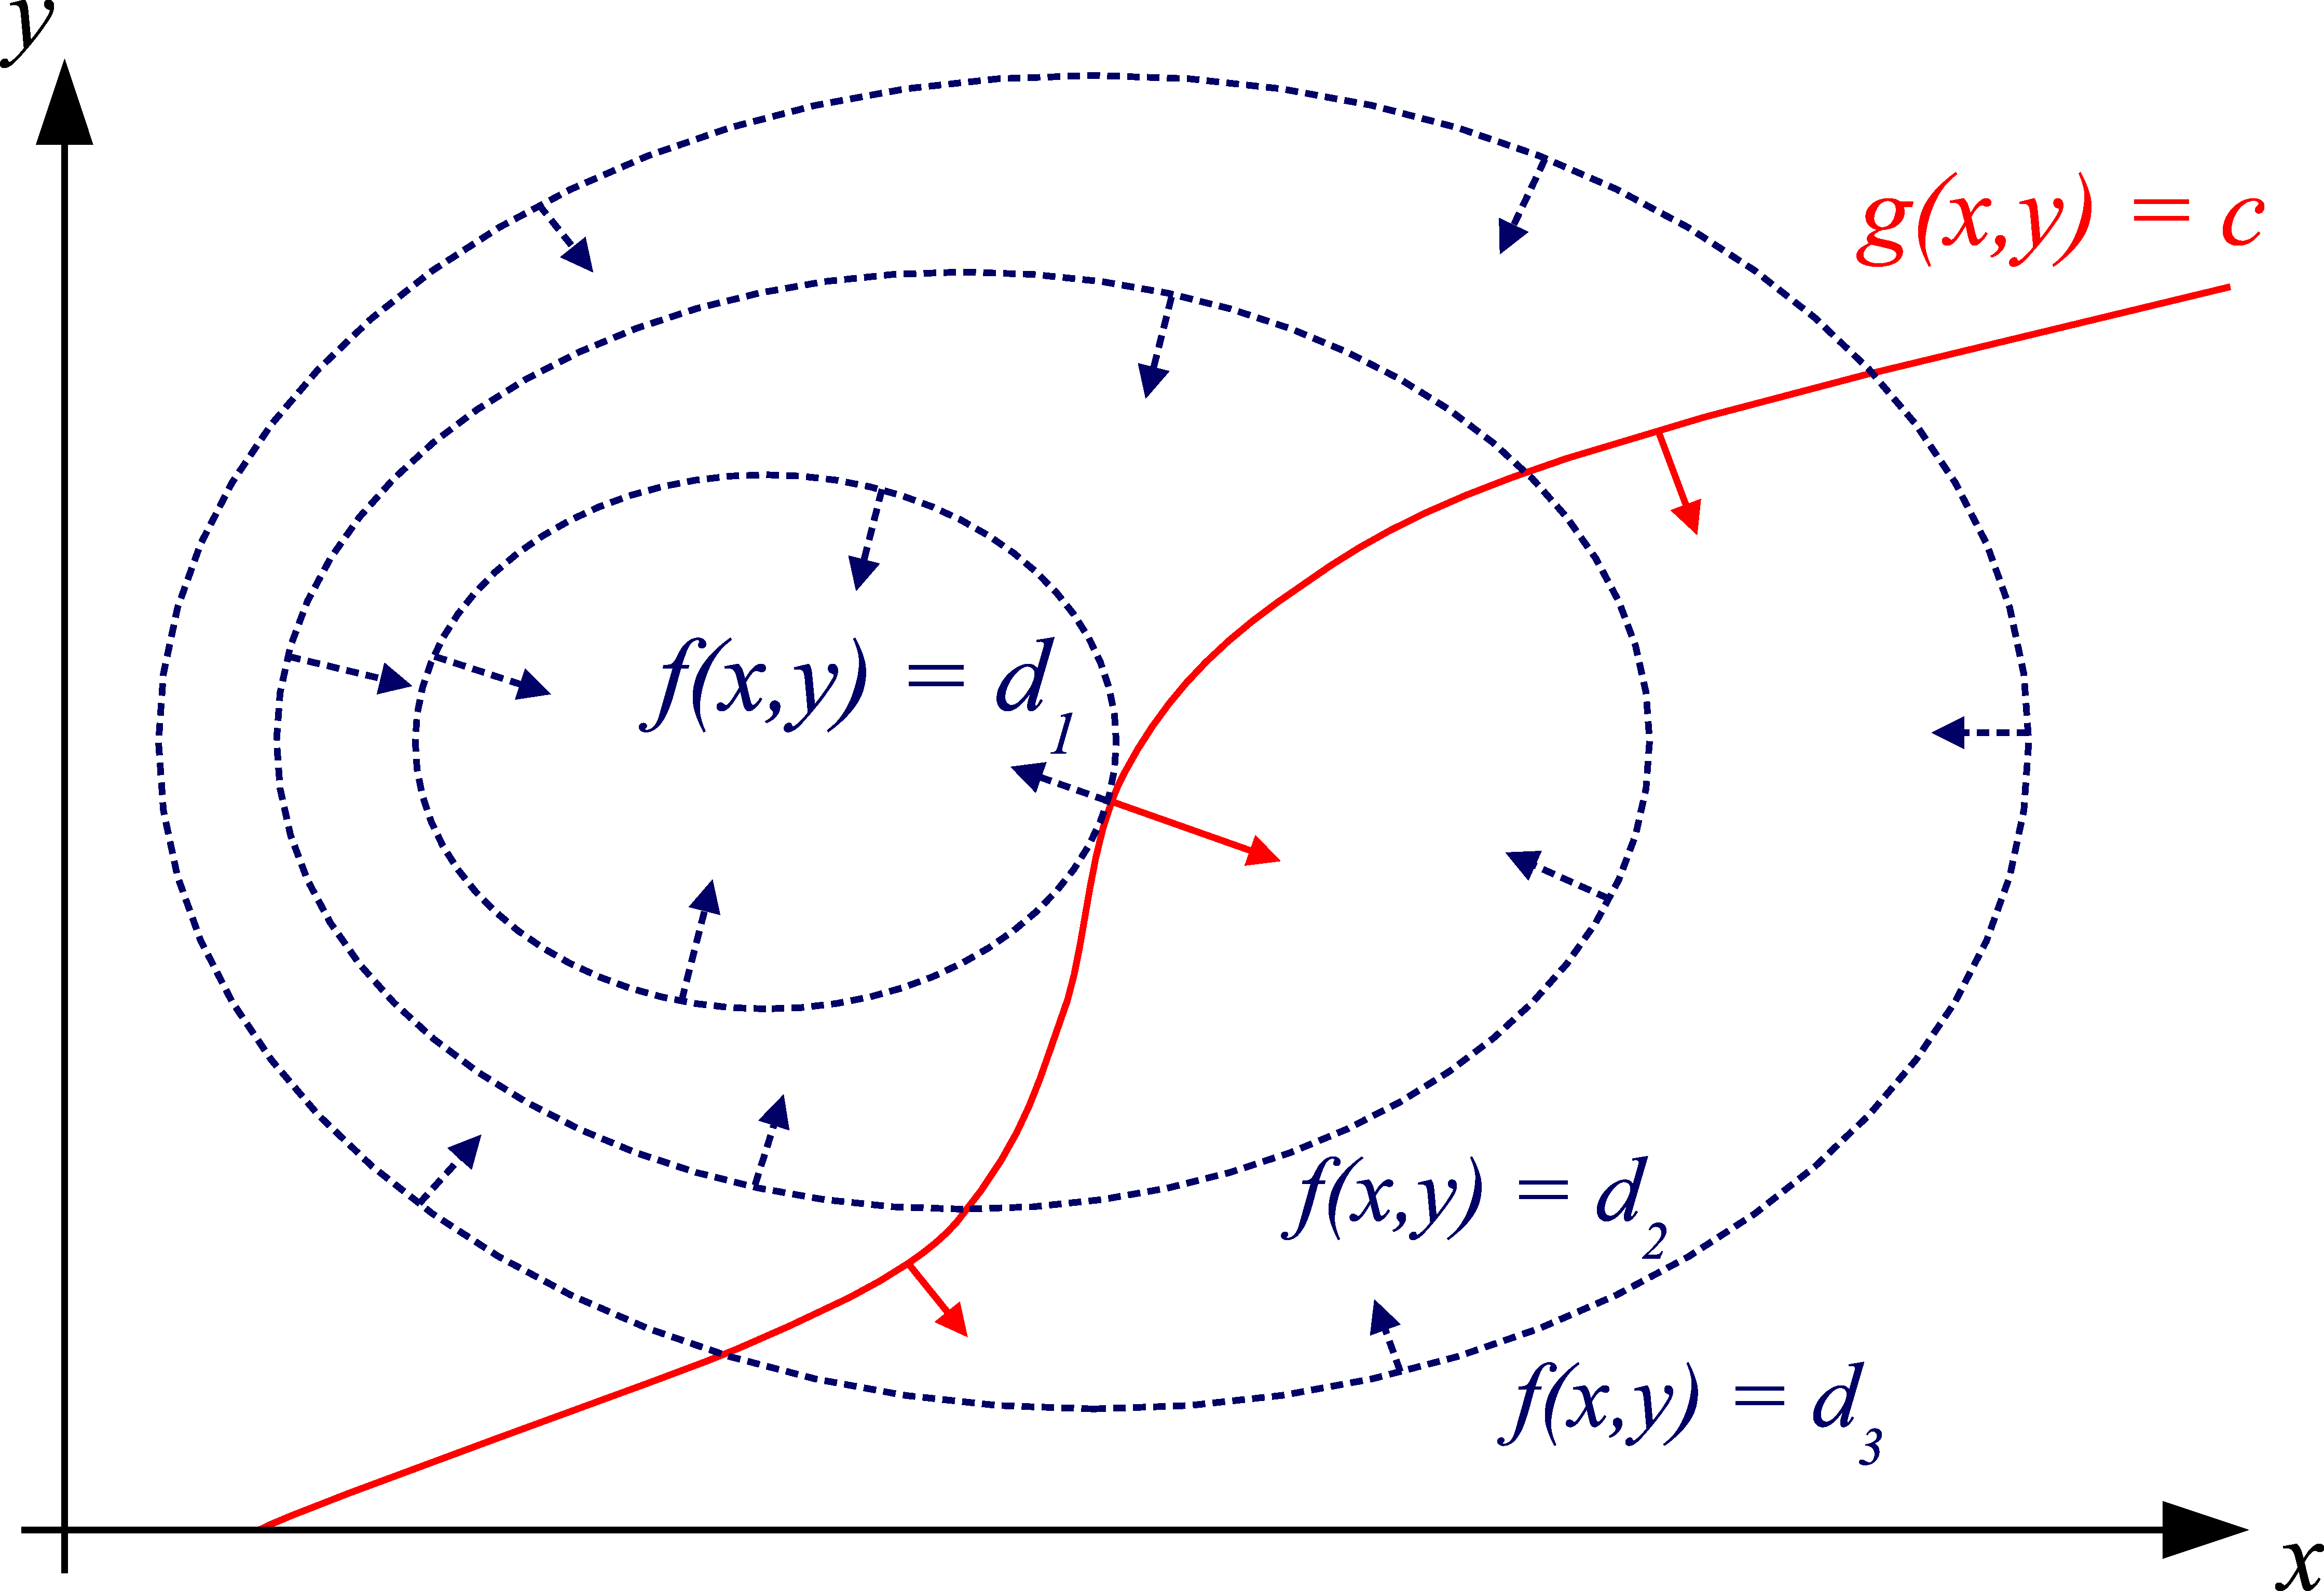
\includegraphics[width=0.6\textwidth]{figs/LagrangeMultipliers2D.pdf}
\end{center}
If the gradients were not parallel, we could move along $g(x,y)=c$ to a higher contour of $f(x,y)$ by following the component of $\nabla f$ parallel to $g(x,y)=c$.


\newpage
\section{Appendix: Optimizing Functionals}
\label{optimizing-functionals}
In order to optimize $\ip{\F|\op{H}_e|\F}$ with respect to variation of the spin MOs, we need to learn how to take a derivative of a functional with respect to a function (a {\it functional derivative} \footnote{\url{http://en.wikipedia.org/wiki/Functional_derivative}}).
First, consider the definition of the derivative of a simple 1D function $f(x)$.
\begin{align*}
	\fr{df(x)}{dx}
\equiv
\lim_{\e\rightarrow0}
	\fr{f(x+\e)-f(x)}{\e}
\end{align*}
which is simply looking at how $f(x)$ changes when we add ``a little bit'' $\e$ of the number $1$.
The stationarity condition for a function is that it doesn't change when we add ``a little bit'' to its argument.
\begin{align}
\lim_{\e\rightarrow0}
	\fr{f(x+\e)-f(x)}{\e}
\overset{!}=0
\end{align}
The stationarity condition of a functional is similar.
To optimize a functional $F[f]$, we require that it doesn't change when we add ``a little bit'' $\e$ of an arbitrary function $g$.
\begin{align}
\lim_{\e\rightarrow0}
	\fr{F[f+\e g]-F[f]}{\e}
\overset{!}=0
\end{align}
Note, however, that $F[f]$ must be stationary with respect to {\it any} form for $g$ -- otherwise we haven't really optimized the thing.

One can (you should) show that that a single derivative may also be written as
\begin{align}
	\fr{df(x)}{dx}
=&\
\left.
	\fr{df(x+\e)}{d\e}
\right|_{\e=0}
\end{align}
by expanding $f$ on the right side in a Taylor series and evaluating the derivative.
This latter form of derivative readily generalizes to functionals.
\begin{align}
\lim_{\e\rightarrow0}
	\fr{F[f+\e g]-F[f]}{\e}
=
\left.
	\fr{dF[f+\e g]}{d\e}
\right|_{\e=0}
\end{align}
and is particularly convenient because it allows us to deal with a plain ol' derivative rather than something more complicated.
Hence, we can obtain stationarity conditions for functionals by requiring that
\begin{align}
\left.
	\fr{dF[f+\e g]}{d\e}
\right|_{\e=0}
\overset{!}=
	0
\end{align}
for {\it any} possible choice of $g$.

\newpage
\section{Appendix: Fundamental Lemma of Calculus of Variations}
\label{flcv}
The {\it Fundamental Lemma of Calculus of Variations} \footnote{\url{http://en.wikipedia.org/wiki/Fundamental_lemma_of_calculus_of_variations}} allows us to deal with situations like
\begin{align}
	\int_{-\infty}^\infty dx f(x)\eta(x)
=
	0
\sp\text{ for all $\eta(x)$}
\end{align}
and tells us that this can only be true if the function $f(x)$ is vanishes everywhere -- that is, if $f(x)=0$.
We can see that this is true by considering the case $\eta(x)=f(x)$.
Since $f(x)^2$ is nonnegative everywhere, the integral can only be zero in this case if $f(x)=0$.

\paragraph{Complex functions.}
Consider an analogous situation for two complex functions $f$ and $g$ that satisfy
\begin{align}
\label{eta}
\int_{-\infty}^\infty dx\
	\eta^*(x)f(x)
+\int_{-\infty}^\infty dx\
	\eta(x)g(x)
=
	0
\sp\text{ for all $\eta(x)$.}
\end{align}
We can show that this can only be satisfied if both $f(x)$ and $g(x)$ separately vanish everywhere. Since $\eta(x)$ is arbitrary, this equation must hold for some other function $\gamma(x) = i \eta(x)$.
\begin{align}
\int_{-\infty}^\infty dx\
	\gamma^*(x)f(x)
+\int_{-\infty}^\infty dx\
	\gamma(x)g(x)
&=
	0
\\[1ex]
\int_{-\infty}^\infty dx\
	[i \eta(x) ]^* f(x)
+\int_{-\infty}^\infty dx\
	[i \eta(x)] g(x)
&=
	0
\\[1ex]
   \label{ieta}
    -i 
    \int_{-\infty}^\infty dx\
	\eta^*(x)  f(x)
+ 
    i \int_{-\infty}^\infty dx\
	\eta(x) g(x)
&=
	0
\end{align}
Adding $i$ times equation (\ref{ieta}) to equation (\ref{eta}) yields:
\begin{equation}
   \label{idk}
	\int_{-\infty}^\infty dx\ 
	\eta^*(x)f(x)=0
\sp\text{ for all $\eta(x)$.}
\end{equation}
Subtracting $i$ times equation (\ref{ieta}) to equation (\ref{eta}) yields:
\begin{equation}
   \label{idk2}
	\int_{-\infty}^\infty dx\ \eta(x)g(x)=0
\sp\text{ for all $\eta(x)$.}
\end{equation}
Again by the Fundamental Lemma of Calculus of Variations, equations (\ref{idk}) and (\ref{idk2}) can only hold true together if $f(x)=0$ and $g(x)=0$.\footnote{Since we could always choose $\eta(x)=f(x)$ or $\eta(x)=g^*(x)$, giving integrands $|f(x)|^2$ and $|g(x)|^2$ that are nonnegative everywhere.}


\newpage
\section{Appendix: Unitary Invariances for Hartree-Fock Orbitals}
\label{hf-invariance}

\paragraph{orbital orthonormality}
Unitary transformations actually always preserve orthonormality by definition, but we can show it:
\begin{align*}
	\ip{\tl\y_i|\tl\y_j}
=
\sum_{kl}
	U_{ki}U_{lj}^*
	\ip{\y_k|\y_l}
=
\sum_{kl}
	U_{ki}U_{lj}^*
	\d_{kl}
=
\sum_k
	U_{ki}U_{kj}^*
=
	\d_{ij}
\end{align*}
using the fact that $\sum_i U_{ki}U_{kj}^*=(\bo{U}\bo{U}\dg)_{ji}=(\bo{1})_{ji}=\d_{ji}$.

\paragraph{Fock operator}
The orbitals enter only into the Coulomb and exchange part of the Fock operator.
For the Coulomb part, we have
{\small\begin{align*}
\sum_i
	\ip{\tl\y_i(2)|\op{g}(1,2)|\tl\y_i(2)}
=
\sum_{ijk}
	U_{ji}U_{ki}^*
	\ip{\y_j(2)|\op{g}(1,2)|\y_k(2)}
=
\sum_{jk}
	\d_{jk}
	\ip{\y_j(2)|\op{g}(1,2)|\y_k(2)}
=
\sum_j
	\ip{\y_j(2)|\op{g}(1,2)|\y_j(2)}
\end{align*} \underline{}}%
using the fact that $\sum_i U_{ji}U_{ki}^*=\d_{jk}$.
For the exchange part, we have the same thing with a $\op{P}(1,2)$ sandwiched in there.

\paragraph{Hamiltonian expectation value}
The vector notation $\bm\y$ for our orbitals allows us to elegantly express $\F$ and $\tl\F$ as follows.
\begin{align*}
	\F(1,\ld,n)
=
	\tfrac{1}{\sqrt{n!}}
	|\bm\y(1)\cd\bm\y(n)|
\sp\sp
	\tl\F(1,\ld,n)
=
	\tfrac{1}{\sqrt{n!}}
	|\tl{\bm\y}(1)\cd\tl{\bm\y}(n)|
\end{align*}
But note that the matrix $\ma{\tl{\bm\y}(1)\ \cd\ \tl{\bm\y}(n)}$ is simply
\begin{align*}
	\ma{\tl{\bm\y}(1)\ \cd\ \tl{\bm\y}(n)}
=
	\ma{\bo{U}\dg\bm\y(1)\ \cd\ \bo{U}\dg\bm\y(n)}
=
	\bo{U}\dg\ma{\bm\y(1)\ \cd\ \bm\y(n)}
\end{align*}
and so $\tl\F=\det(\bo{U}\dg)\F=\det(\bo{U})^*\F$, which means
\begin{align}
	\ip{\tl\F|\op{H}_e|\tl\F}
=
	\det(\bo{U}\bo{U}\dg)\ip{\F|\op{H}_e|\F}
=
	\ip{\F|\op{H}_e|\F}
\end{align}


%end of the document
\end{document}
